\chapter{実装}
\label{chap:implementation}

\section{実装概要}
本研究における実験に必要な実装物について、以下に示す。

\section{インスリンペンデバイス}
\label{section:insulin_pen_device}

インスリン摂取を検知するためのインスリンペンデバイスは以下の機器で構成される。

\subsection{環境}

\begin{table}[htbp]
  \caption{インスリンデバイスの実装環境}
  \label{tb:insulin-device}
  \begin{center}
    \begin{tabular}{c||c}
      \hline
      言語  & C++ \\\hline
      通信機器  & ESP32 devkit v1 \\\hline
      注射器 & 〇〇 \\\hline
    \end{tabular}
  \end{center}
\end{table}

ESP32の画像を貼る。

インスリン注射器の画像を貼る。

インスリン注射器の端のボタンが一定時間以上押された場合に摂取と判定する構造を作るため、被験者の親指を伝導物として見立て、一定以上マイコンが電流が流れたことを感知した場合に、
インスリンが摂取されたとして判定するよう実装した。

本論文ではマイクロコンピュータが感知できる電圧〇〇を閾値として検知を行った。
他にも〇〇、〇〇に関しても実験を行った結果、以上の値が適切であると判断した。

図\ref{fig:insulin_pen_device_circuit}に、ESP32とそのスイッチ回路を示す。

\begin{figure}[htbp]
  \caption{インスリン注射器に装着するデバイスの回路}
  \label{fig:insulin_pen_device_circuit}
  \begin{center}
    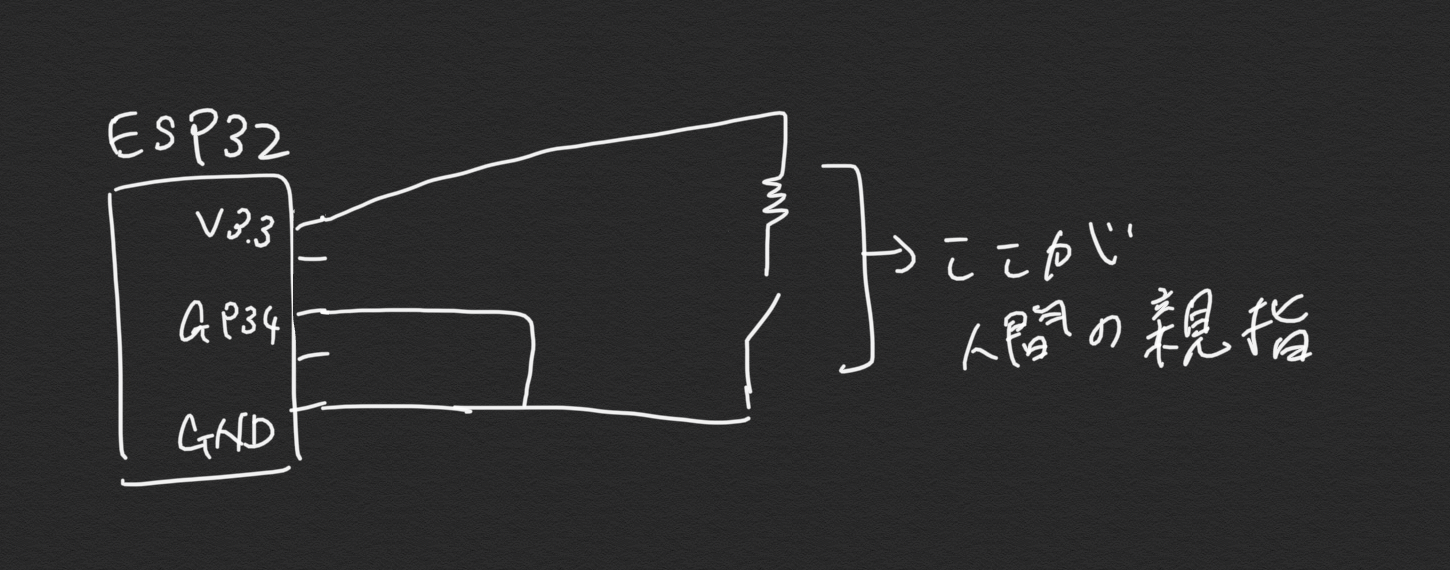
\includegraphics[bb=0 0 1000 300,width=20cm]{assets/insulin_pen_device_circuit.png}
  \end{center}
\end{figure}


インスリンペンについたデバイスがどのような電子回路になっているか載せる。

回路のスイッチの部分が、タクトスイッチなどではなく、あくまで人間の親指になるのが本実装である。
抵抗値に関しては実際に実装済みのもので実験をすることで、どれほどの値になるかを計測した。

図\ref{}が実際の実装物である。小型化し、電池により携帯可能にする段階は本研究の本質ではないため、今回の実装内容としては省いた。

実際のインスリンペンとデバイスがくっついている感じのものを見せる

実際のインスリン摂取時間は、raspberry piにホストしたwebサーバーを介して、MySQLのデータベースに保存している。
このリクエストを受けるraspberry piは後に食事検知にも使用されているRaspberry Pi 4 Model Bである。
実際にインスリン注射器の端が親指で押され、抵抗値が○○以上になり、マイクロコンピュータに流れる電圧が〇〇になると、
HTTPのPOSTリクエストを投げる仕組みである。

\ref{}にこの実装部分の概略と、フローを示す。

\section{食事検知加速度センサ}

今回、食事の検知は食卓上に鎮座させる加速度センサによる手法を採用した。検知デバイスは以下の機器で構成されている。

\subsection{使用機器}

\begin{table}[htbp]
  \caption{食事検知に使用したセンサー及びPC}
  \label{tb:meal_detection_spec}
  \begin{center}
    \begin{tabular}{c||c}
      \hline
      加速度センサ & ADXL345 \\\hline
      PC & Raspberry Pi 4 Model B (SD: 32GB) \\\hline
    \end{tabular}
  \end{center}
\end{table}

加速度センサの画像を貼る。

ADXL345は3軸加速度センサであり、縦、横、高さの3つの値を取得することができる。

ラズパイ4の画像貼る。

??に、本研究で使用したRaspberry Piのスペックを示す。

\begin{table}[htbp]
  \caption{Raspberry Piのスペック}
  \label{tb:raspberry_pi_spec}
  \begin{center}
    \begin{tabular}{c||c}
      \hline
      OS  & Raspbian GNU/Linux 10 (buster) \\\hline
      CPU & Broadcom BCM2711, quad-core Cortex-A72 (ARM v8) 64-bit SoC @ 1.5GHz \\\hline
      RAM & 4GB \\\hline
    \end{tabular}
  \end{center}
\end{table}

raspberry piで加速度センサの値を読めるようになるための実装説明

配線図をここに書く。

実物の写真をここに貼る。

加速度センサでどういう値が取れるのかをmatplotlibで可視化したやつそのまま貼って説明。

どんな条件で食事検知とするのかを書く。

\section{インスリン打ち忘れ通知}

どうしたら打ち忘れとして通知に至るのかのフローを示す。

\begin{figure}[htbp]
  \caption{インスリン摂取忘れ通知フロー}
  \label{fig:system_flow}
  \begin{center}
    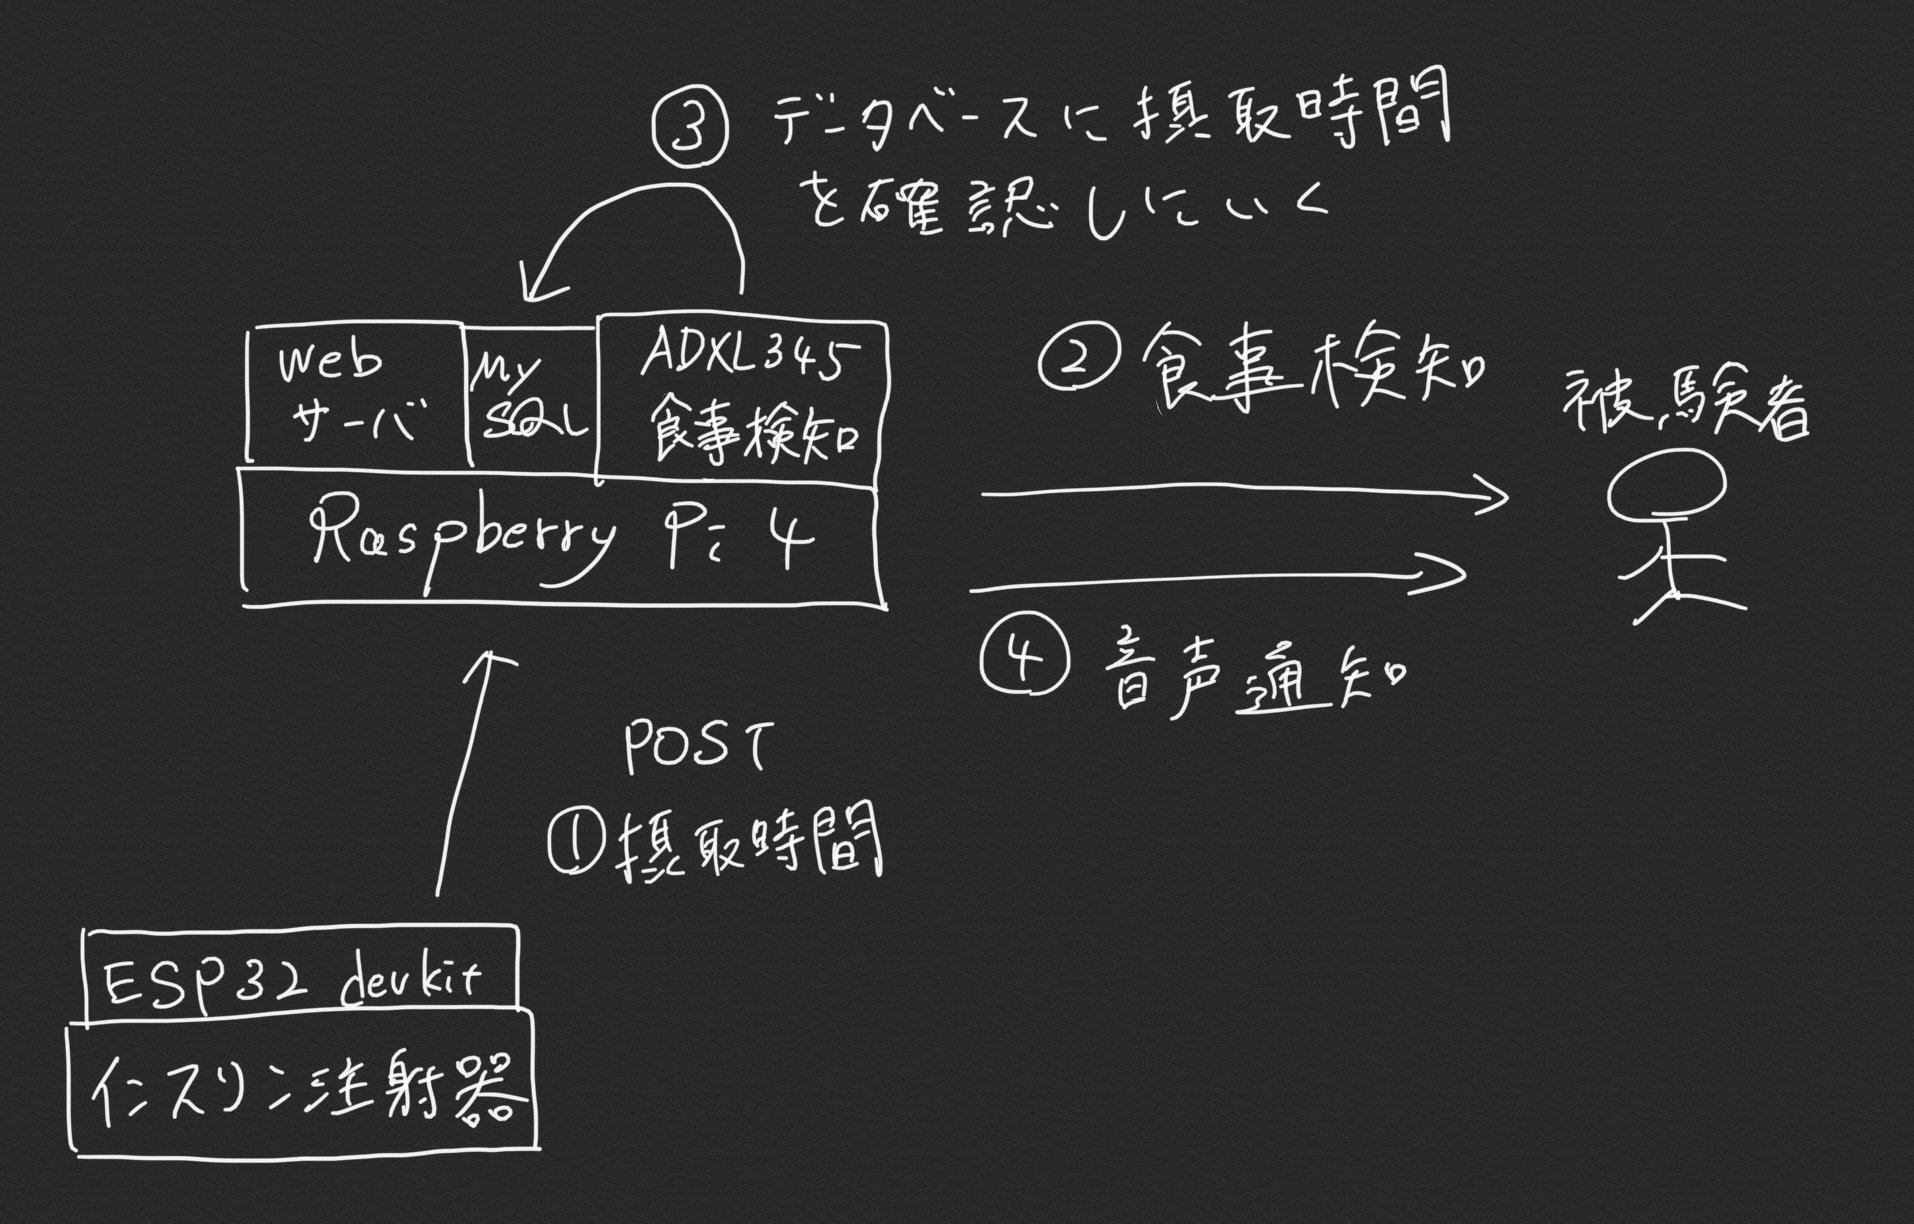
\includegraphics[bb=0 0 1000 600,width=15cm]{assets/system_flow.png}
  \end{center}
\end{figure}
